\documentclass[12pt]{article}
\usepackage[a4paper,margin=1in]{geometry}
\usepackage{amsmath,amssymb}
\usepackage{graphicx}
\usepackage{siunitx}
\sisetup{per-mode=symbol}
\usepackage{gvv}

\title{Matrix 2.10.4}
\author{ai25btech11015 -- M Sai Rithik}
\date{}

\begin{document}
\maketitle

\section*{Question}
Find the area of the triangle whose vertices are 
\[
A(1,-1,2), \quad B(2,0,-1), \quad C(3,-1,2).
\]

\section*{Solution}

\subsection*{Step 1: Form vectors}
\begin{align}
\Vec{B}-\Vec{A} &= \myvec{2-1 \\ 0-(-1) \\ -1-2} = \myvec{1 \\ 1 \\ -3}, \tag{1}\\
\Vec{C}-\Vec{A} &= \myvec{3-1 \\ -1-(-1) \\ 2-2} = \myvec{2 \\ 0 \\ 0}. \tag{2}
\end{align}

\subsection*{Step 2: Cross product formula}
The cross product of two vectors is defined as
\begin{align}
\Vec{X}\times\Vec{Y} =
\myvec{
  \mydet{\Vec{X}_{23} & \Vec{Y}_{23}} \\
  \mydet{\Vec{X}_{31} & \Vec{Y}_{31}} \\
  \mydet{\Vec{X}_{12} & \Vec{Y}_{12}}
}. \tag{3}
\end{align}

Applying to $\Vec{B}-\Vec{A}$ and $\Vec{C}-\Vec{A}$:
\begin{align}
(\Vec{B}-\Vec{A})\times(\Vec{C}-\Vec{A})
&= 
\myvec{
\mydet{\myvec{1 \\ -3} & \myvec{0 \\ 0}} \\
\mydet{\myvec{-3 \\ 1} & \myvec{0 \\ 2}} \\
\mydet{\myvec{1 \\ 1} & \myvec{2 \\ 0}}
}. \tag{4}
\end{align}

\subsection*{Step 3: Simplify}
\begin{align}
(\Vec{B}-\Vec{A})\times(\Vec{C}-\Vec{A})
&= \myvec{
(1)(0) - (-3)(0) \\
(-3)(2) - (1)(0) \\
(1)(0) - (1)(2)
} \\
&= \myvec{0 \\ -6 \\ -2}. \tag{5}
\end{align}

\subsection*{Step 4: Area of triangle}
\begin{align}
\text{Area of } \triangle ABC &= \tfrac{1}{2}\left\|(\Vec{B}-\Vec{A})\times(\Vec{C}-\Vec{A})\right\| \\
&= \tfrac{1}{2}\sqrt{0^2+(-6)^2+(-2)^2} \\
&= \tfrac{1}{2}\sqrt{40} \\
&= \sqrt{10}. \tag{6}
\end{align}

\section*{Final Answer}
\[
\boxed{\text{Area of } \triangle ABC = \sqrt{10}}
\]

\begin{figure}[h!]
    \centering
    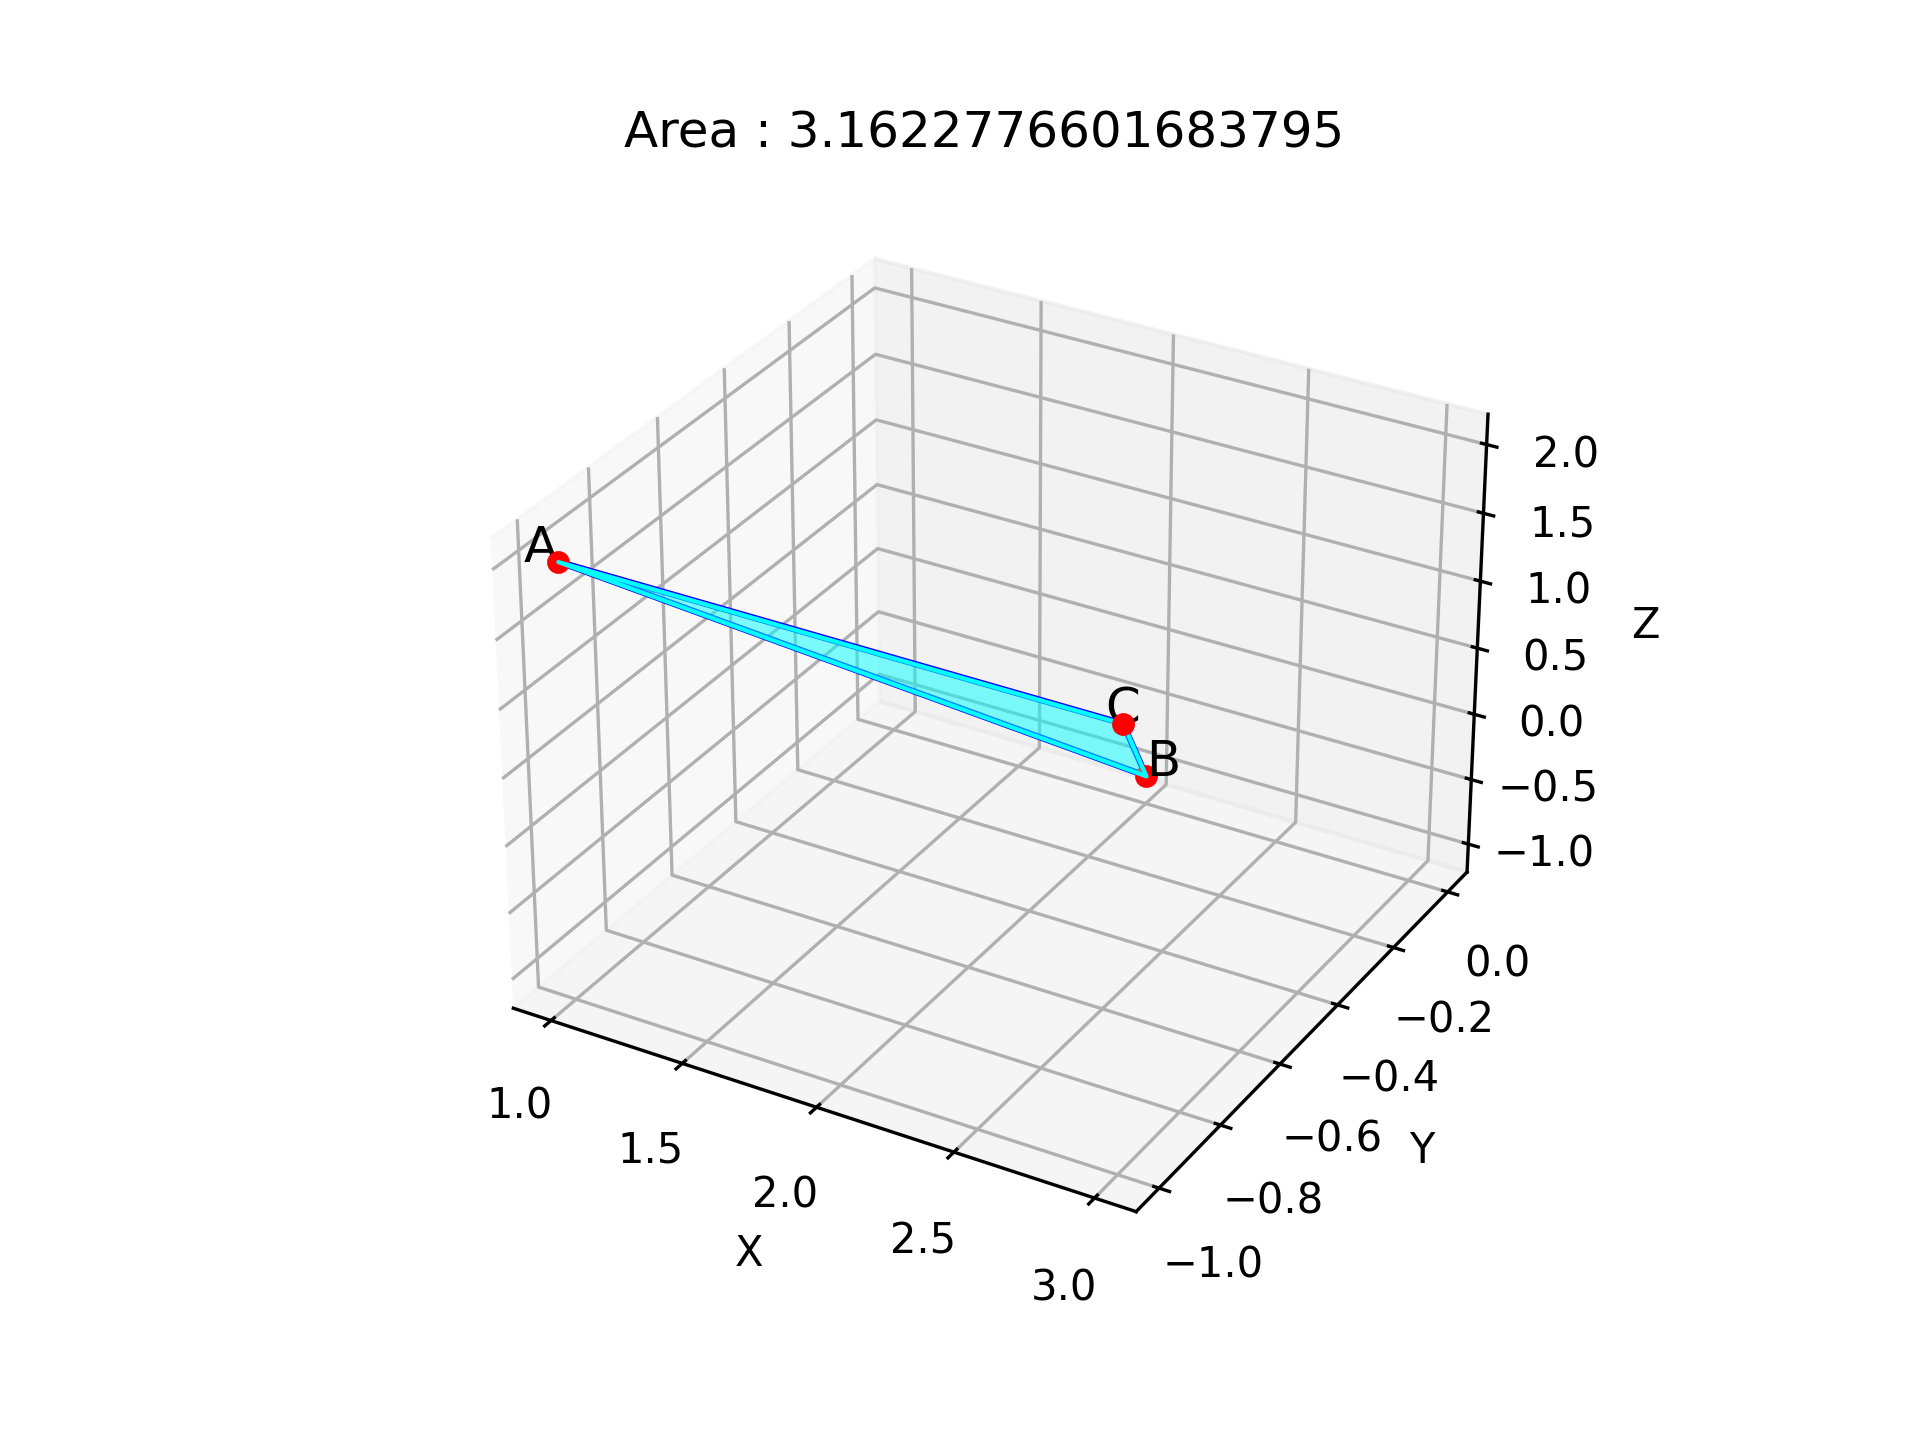
\includegraphics[width=0.65\linewidth]{figs/fig.png}
    \caption{Triangle formed by points $A$, $B$, and $C$.}
\end{figure}

\end{document}
